\documentclass[border=25pt]{standalone}
\usepackage{tikz}
\usepackage{xcolor}
\usetikzlibrary{positioning, calc, shapes, arrows.meta}

\definecolor{coreHeader}{HTML}{1565C0}
\definecolor{coreFill}{HTML}{E3F2FD}
\definecolor{eventHeader}{HTML}{2E7D32}
\definecolor{eventFill}{HTML}{E8F5E9}
\definecolor{commHeader}{HTML}{6A1B9A}
\definecolor{commFill}{HTML}{F3E5F5}
\definecolor{payHeader}{HTML}{EF6C00}
\definecolor{payFill}{HTML}{FFF3E0}
\definecolor{notifHeader}{HTML}{37474F}
\definecolor{notifFill}{HTML}{ECEFF1}
\definecolor{borderdark}{HTML}{212121}
\definecolor{linecolor}{HTML}{000000}

\begin{document}
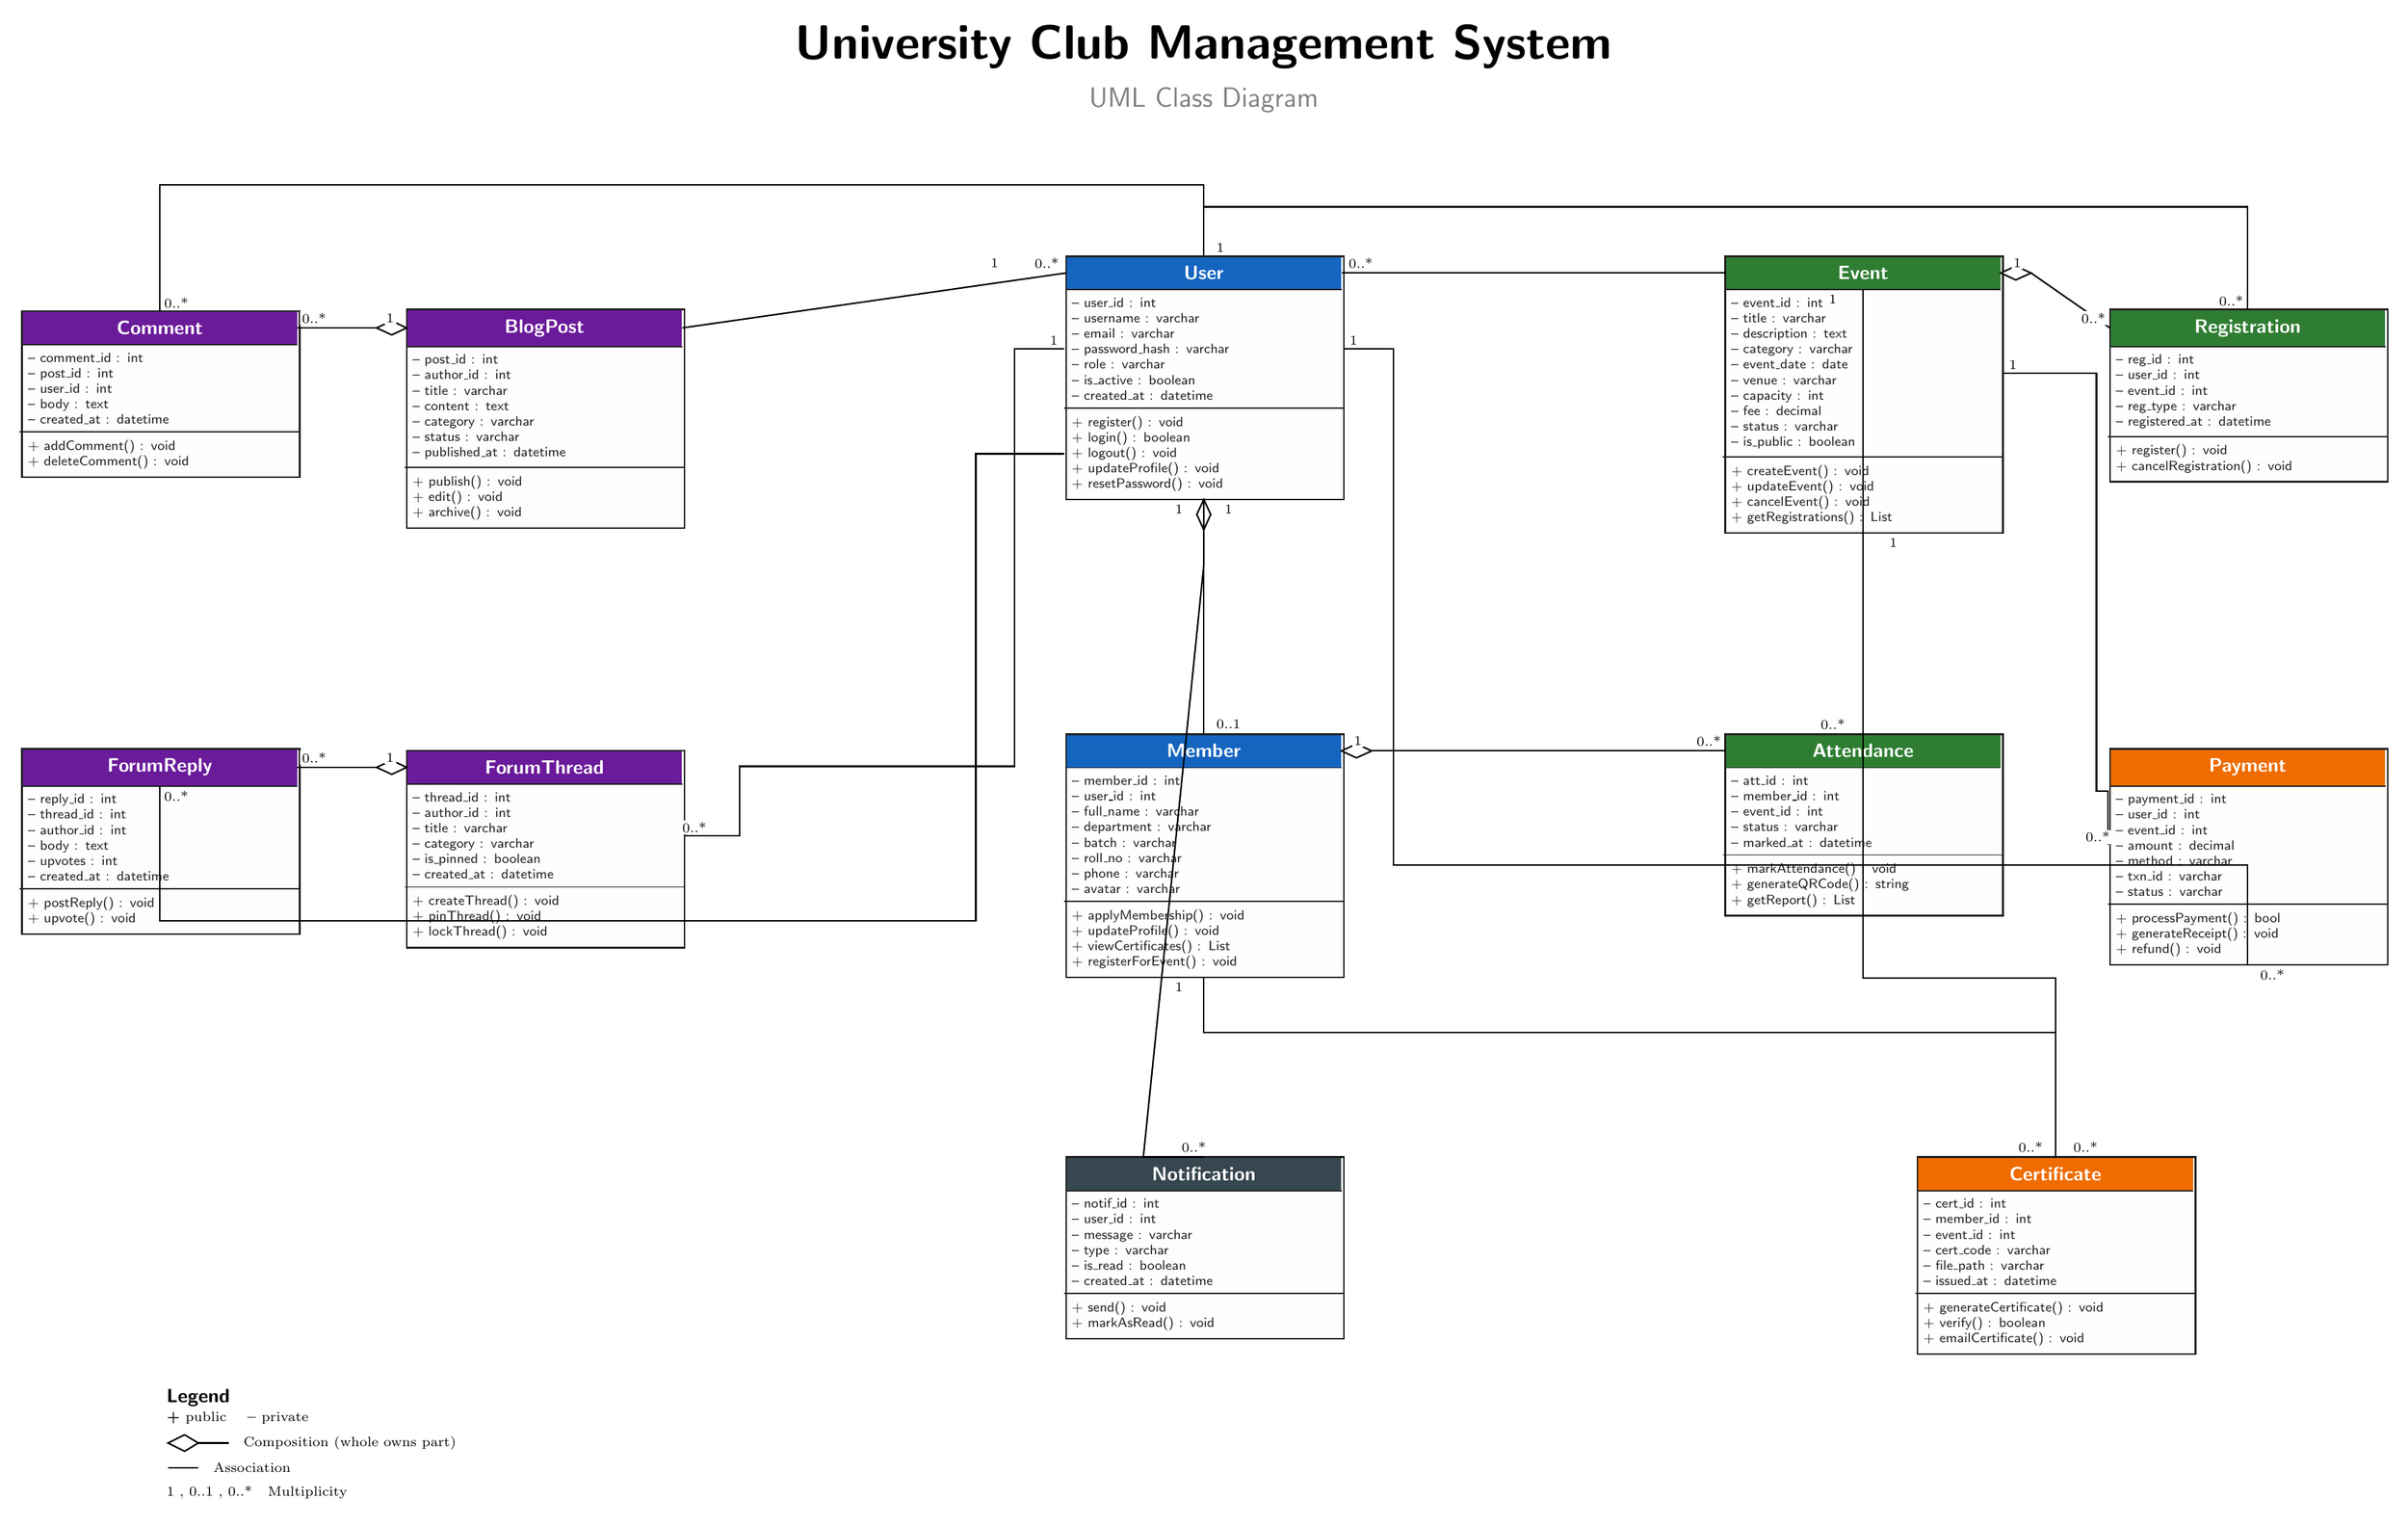
\begin{tikzpicture}[font=\sffamily, every node/.style={font=\sffamily}]

\tikzset{
  cls header/.style={rectangle, minimum width=5.0cm, fill=#1, text=white,
    font=\sffamily\bfseries\normalsize, align=center, draw=none, inner sep=5pt},
  cls section/.style={rectangle, minimum width=5.0cm, fill=#1!10!white,
    text=borderdark, font=\sffamily\scriptsize, align=left, draw=none, inner sep=4pt},
}

%% Macro to draw a complete class box.
%% #1=node-id-prefix #2=(x,y) #3=header color #4=fill color #5=title #6=attribute lines #7=method lines
\newcommand{\umlclass}[7]{%
  \node[cls header=#3] (#1-h) at #2 {#5};
  \node[cls section=#4, anchor=north, align=left, text width=4.8cm] (#1-a) at (#1-h.south) {#6};
  \node[cls section=#4, anchor=north, align=left, text width=4.8cm] (#1-m) at (#1-a.south) {#7};
  \draw[borderdark, line width=0.9pt] (#1-h.north west) rectangle (#1-m.south east);
  \draw[borderdark, line width=0.6pt] (#1-h.south west) -- (#1-h.south east);
  \draw[borderdark, line width=0.6pt] (#1-a.south west) -- (#1-a.south east);
}

% ════════════════════════════════════════════════════════════════════════
% GRID LAYOUT  (column x-positions: -19, -12.5, -6, 0, 6, 12.5, 19)
% Row y-positions chosen with generous gaps based on content height
% ════════════════════════════════════════════════════════════════════════

% ---- Row 1 (top): COMMENT | BLOGPOST |        | USER        |        | EVENT       | REGISTRATION
\umlclass{com}{(-19,20)}{commHeader}{commFill}{Comment}{
  -- comment\_id : int\\ -- post\_id : int\\ -- user\_id : int\\ -- body : text\\ -- created\_at : datetime
}{
  + addComment() : void\\ + deleteComment() : void
}

\umlclass{blog}{(-12,20)}{commHeader}{commFill}{BlogPost}{
  -- post\_id : int\\ -- author\_id : int\\ -- title : varchar\\ -- content : text\\
  -- category : varchar\\ -- status : varchar\\ -- published\_at : datetime
}{
  + publish() : void\\ + edit() : void\\ + archive() : void
}

\umlclass{user}{(0,21)}{coreHeader}{coreFill}{User}{
  -- user\_id : int\\ -- username : varchar\\ -- email : varchar\\ -- password\_hash : varchar\\
  -- role : varchar\\ -- is\_active : boolean\\ -- created\_at : datetime
}{
  + register() : void\\ + login() : boolean\\ + logout() : void\\
  + updateProfile() : void\\ + resetPassword() : void
}

\umlclass{ev}{(12,21)}{eventHeader}{eventFill}{Event}{
  -- event\_id : int\\ -- title : varchar\\ -- description : text\\ -- category : varchar\\
  -- event\_date : date\\ -- venue : varchar\\ -- capacity : int\\ -- fee : decimal\\
  -- status : varchar\\ -- is\_public : boolean
}{
  + createEvent() : void\\ + updateEvent() : void\\ + cancelEvent() : void\\ + getRegistrations() : List
}

\umlclass{reg}{(19,20)}{eventHeader}{eventFill}{Registration}{
  -- reg\_id : int\\ -- user\_id : int\\ -- event\_id : int\\ -- reg\_type : varchar\\ -- registered\_at : datetime
}{
  + register() : void\\ + cancelRegistration() : void
}

% ---- Row 2 (middle): FORUMREPLY | FORUMTHREAD |  | MEMBER |  | ATTENDANCE | PAYMENT
\umlclass{rep}{(-19,12)}{commHeader}{commFill}{ForumReply}{
  -- reply\_id : int\\ -- thread\_id : int\\ -- author\_id : int\\ -- body : text\\
  -- upvotes : int\\ -- created\_at : datetime
}{
  + postReply() : void\\ + upvote() : void
}

\umlclass{th}{(-12,12)}{commHeader}{commFill}{ForumThread}{
  -- thread\_id : int\\ -- author\_id : int\\ -- title : varchar\\ -- category : varchar\\
  -- is\_pinned : boolean\\ -- created\_at : datetime
}{
  + createThread() : void\\ + pinThread() : void\\ + lockThread() : void
}

\umlclass{mem}{(0,12.3)}{coreHeader}{coreFill}{Member}{
  -- member\_id : int\\ -- user\_id : int\\ -- full\_name : varchar\\ -- department : varchar\\
  -- batch : varchar\\ -- roll\_no : varchar\\ -- phone : varchar\\ -- avatar : varchar
}{
  + applyMembership() : void\\ + updateProfile() : void\\
  + viewCertificates() : List\\ + registerForEvent() : void
}

\umlclass{att}{(12,12.3)}{eventHeader}{eventFill}{Attendance}{
  -- att\_id : int\\ -- member\_id : int\\ -- event\_id : int\\ -- status : varchar\\ -- marked\_at : datetime
}{
  + markAttendance() : void\\ + generateQRCode() : string\\ + getReport() : List
}

\umlclass{pay}{(19,12)}{payHeader}{payFill}{Payment}{
  -- payment\_id : int\\ -- user\_id : int\\ -- event\_id : int\\ -- amount : decimal\\
  -- method : varchar\\ -- txn\_id : varchar\\ -- status : varchar
}{
  + processPayment() : bool\\ + generateReceipt() : void\\ + refund() : void
}

% ---- Row 3 (bottom): | | NOTIFICATION (under Member) | | CERTIFICATE (under Attendance/Payment)
\umlclass{not}{(0,4.6)}{notifHeader}{notifFill}{Notification}{
  -- notif\_id : int\\ -- user\_id : int\\ -- message : varchar\\ -- type : varchar\\
  -- is\_read : boolean\\ -- created\_at : datetime
}{
  + send() : void\\ + markAsRead() : void
}

\umlclass{cert}{(15.5,4.6)}{payHeader}{payFill}{Certificate}{
  -- cert\_id : int\\ -- member\_id : int\\ -- event\_id : int\\ -- cert\_code : varchar\\
  -- file\_path : varchar\\ -- issued\_at : datetime
}{
  + generateCertificate() : void\\ + verify() : boolean\\ + emailCertificate() : void
}

% ════════════════════════════════════════════════════════════════════════
% RELATIONSHIP MACROS
% ════════════════════════════════════════════════════════════════════════
\newcommand{\diamondmark}[3]{%
  \fill[#3, draw=linecolor, line width=0.8pt]
    (#1) -- ($(#1)+(#2+25:0.30)$) -- ($(#1)+(#2:0.55)$) -- ($(#1)+(#2-25:0.30)$) -- cycle;
}

\begin{scope}[every path/.style={line width=0.8pt, draw=linecolor}]

% USER -- MEMBER : Composition, vertical
\diamondmark{user-m.south}{-90}{white}
\draw ($(user-m.south)+(0,-0.55)$) -- (mem-h.north);
\node[font=\scriptsize, fill=white, inner sep=1pt] at ($(user-m.south)+(0.45,-0.18)$) {1};
\node[font=\scriptsize, fill=white, inner sep=1pt] at ($(mem-h.north)+(0.45,0.18)$) {0..1};

% USER -- NOTIFICATION : straight vertical (Notification sits directly below User column)
\draw (user-m.south) -- ++(0,-1.2) -- ($(not-h.north)+(-1.1,0)$) -- (not-h.north);
\node[font=\scriptsize, fill=white, inner sep=1pt] at ($(user-m.south)+(-0.45,-0.18)$) {1};
\node[font=\scriptsize, fill=white, inner sep=1pt] at ($(not-h.north)+(-0.18,0.18)$) {0..*};

% USER -- EVENT : Association
\draw (user-h.east) -- (ev-h.west);
\node[font=\scriptsize, fill=white, inner sep=1pt] at ($(user-h.east)+(0.35,0.18)$) {0..*};

% USER -- REGISTRATION : Association, routed above User/Event row
\draw (user-h.north) -- ++(0,0.9) -| (reg-h.north);
\node[font=\scriptsize, fill=white, inner sep=1pt] at ($(user-h.north)+(0.30,0.15)$) {1};
\node[font=\scriptsize, fill=white, inner sep=1pt] at ($(reg-h.north)+(-0.30,0.15)$) {0..*};

% USER -- PAYMENT : Association, routed below row (through gap)
\draw (user-a.east) -- ++(0.9,0) -- ++(0,-9.4) -| (pay-m.south);
\node[font=\scriptsize, fill=white, inner sep=1pt] at ($(user-a.east)+(0.18,0.15)$) {1};
\node[font=\scriptsize, fill=white, inner sep=1pt] at ($(pay-m.south)+(0.45,-0.18)$) {0..*};

% USER -- BLOGPOST : Association
\draw (user-h.west) -- (blog-h.east);
\node[font=\scriptsize, fill=white, inner sep=1pt] at ($(user-h.west)+(-0.35,0.18)$) {0..*};
\node[font=\scriptsize, fill=white, inner sep=1pt] at ($(user-h.west)+(-1.3,0.18)$) {1};

% USER -- COMMENT : Association routed above row
\draw (user-h.north) -- ++(0,1.3) -| (com-h.north);
\node[font=\scriptsize, fill=white, inner sep=1pt] at ($(com-h.north)+(0.30,0.15)$) {0..*};

% USER -- FORUMTHREAD : Association, routed below row, enters from the right edge
\draw (user-a.west) -- ++(-0.9,0) -- ++(0,-7.6) -| ($(th-a.east)+(1.0,0)$) -- (th-a.east);
\node[font=\scriptsize, fill=white, inner sep=1pt] at ($(user-a.west)+(-0.18,0.15)$) {1};
\node[font=\scriptsize, fill=white, inner sep=1pt] at ($(th-a.east)+(0.18,0.15)$) {0..*};

% USER -- FORUMREPLY : Association, routed further below
\draw (user-m.west) -- ++(-1.6,0) -- ++(0,-8.5) -| (rep-h.south);
\node[font=\scriptsize, fill=white, inner sep=1pt] at ($(rep-h.south)+(0.30,-0.18)$) {0..*};

% MEMBER -- ATTENDANCE : Composition
\diamondmark{mem-h.east}{0}{white}
\draw ($(mem-h.east)+(0.55,0)$) -- (att-h.west);
\node[font=\scriptsize, fill=white, inner sep=1pt] at ($(mem-h.east)+(0.30,0.18)$) {1};
\node[font=\scriptsize, fill=white, inner sep=1pt] at ($(att-h.west)+(-0.30,0.18)$) {0..*};

% MEMBER -- CERTIFICATE : Composition, routed below
\draw (mem-m.south) -- ++(0,-1.0) -| (cert-h.north);
\node[font=\scriptsize, fill=white, inner sep=1pt] at ($(mem-m.south)+(-0.45,-0.18)$) {1};
\node[font=\scriptsize, fill=white, inner sep=1pt] at ($(cert-h.north)+(-0.45,0.18)$) {0..*};

% EVENT -- REGISTRATION : Composition
\diamondmark{ev-h.east}{0}{white}
\draw ($(ev-h.east)+(0.55,0)$) -- (reg-h.west);
\node[font=\scriptsize, fill=white, inner sep=1pt] at ($(ev-h.east)+(0.30,0.18)$) {1};
\node[font=\scriptsize, fill=white, inner sep=1pt] at ($(reg-h.west)+(-0.30,0.18)$) {0..*};

% EVENT -- ATTENDANCE : Association, vertical
\draw (ev-h.south) -- ++(0,-7.6) -- (att-h.north);
\node[font=\scriptsize, fill=white, inner sep=1pt] at ($(ev-h.south)+(-0.55,-0.18)$) {1};
\node[font=\scriptsize, fill=white, inner sep=1pt] at ($(att-h.north)+(-0.55,0.18)$) {0..*};

% EVENT -- PAYMENT : Association, vertical
\draw (ev-a.east) -- ++(1.7,0) -- ++(0,-7.6) -| (pay-a.west);
\node[font=\scriptsize, fill=white, inner sep=1pt] at ($(ev-a.east)+(0.18,0.15)$) {1};
\node[font=\scriptsize, fill=white, inner sep=1pt] at ($(pay-a.west)+(-0.18,0.15)$) {0..*};

% EVENT -- CERTIFICATE : Association
\draw (ev-m.south) -- ++(0,-1.0) -- ++(0,-7.1) -| (cert-h.north);
\node[font=\scriptsize, fill=white, inner sep=1pt] at ($(ev-m.south)+(0.55,-0.18)$) {1};
\node[font=\scriptsize, fill=white, inner sep=1pt] at ($(cert-h.north)+(0.55,0.18)$) {0..*};

% BLOGPOST -- COMMENT : Composition
\diamondmark{blog-h.west}{180}{white}
\draw ($(blog-h.west)+(-0.55,0)$) -- (com-h.east);
\node[font=\scriptsize, fill=white, inner sep=1pt] at ($(blog-h.west)+(-0.30,0.18)$) {1};
\node[font=\scriptsize, fill=white, inner sep=1pt] at ($(com-h.east)+(0.30,0.18)$) {0..*};

% FORUMTHREAD -- FORUMREPLY : Composition
\diamondmark{th-h.west}{180}{white}
\draw ($(th-h.west)+(-0.55,0)$) -- (rep-h.east);
\node[font=\scriptsize, fill=white, inner sep=1pt] at ($(th-h.west)+(-0.30,0.18)$) {1};
\node[font=\scriptsize, fill=white, inner sep=1pt] at ($(rep-h.east)+(0.30,0.18)$) {0..*};

\end{scope}

% ════════════════════════════════════════════════════════════════════════
% LEGEND
% ════════════════════════════════════════════════════════════════════════
\begin{scope}[shift={(-19,0.5)}]
\node[anchor=north west, font=\sffamily\bfseries\normalsize] at (0,0.3) {Legend};
\node[anchor=west, font=\scriptsize] at (0,-0.35) {\textbf{+} public \quad \textbf{--} private};
\fill[white, draw=linecolor, line width=0.8pt]
  (0.15,-0.80) -- (0.45,-0.65) -- (0.70,-0.80) -- (0.45,-0.95) -- cycle;
\draw[line width=0.8pt] (0.70,-0.80) -- (1.25,-0.80);
\node[anchor=west, font=\scriptsize] at (1.4,-0.80) {Composition (whole owns part)};
\draw[line width=0.8pt] (0.15,-1.25) -- (0.70,-1.25);
\node[anchor=west, font=\scriptsize] at (0.85,-1.25) {Association};
\node[anchor=west, font=\scriptsize] at (0,-1.70) {1 ,\ 0..1 ,\ 0..* \ \ Multiplicity};
\end{scope}

% ════════════════════════════════════════════════════════════════════════
% TITLE
% ════════════════════════════════════════════════════════════════════════
\node[anchor=south, font=\sffamily\bfseries\Huge] at (0,24.6) {University Club Management System};
\node[anchor=south, font=\sffamily\Large, gray] at (0,23.8) {UML Class Diagram};

\end{tikzpicture}
\end{document}
